\documentclass[a4paper,12pt]{article}
\usepackage{graphicx}
\usepackage{longtable}
\usepackage{caption}
\usepackage{listings}
\usepackage{color}

\definecolor{dkgreen}{rgb}{0,0.6,0}
\definecolor{gray}{rgb}{0.5,0.5,0.5}
\definecolor{mauve}{rgb}{0.58,0,0.82}

\lstset{frame=tb,
    language=Java,
    aboveskip=3mm,
    belowskip=3mm,
    showstringspaces=false,
    columns=flexible,
    basicstyle={\small\ttfamily},
    numbers=none,
    numberstyle=\tiny\color{gray},
    keywordstyle=\color{blue},
    commentstyle=\color{dkgreen},
    stringstyle=\color{mauve},
    breaklines=true,
    breakatwhitespace=true,
    tabsize=3
}

\title{Lab 2: Interprocess Communications with Pipes and Java Threads}
\author{Liam Geraghty - 300356748 \\ Shane Stock - XXXXXXXXX \\ CSI3131 - Operating Systems \\ 2025-06-08}
\date{}

\begin{document}

\maketitle

\section{Introduction and Objectives}
The objective of this lab is to explore interprocess communication (IPC) using UNIX/Linux pipes and to learn about Java threads and thread pools. The specific goals include:
\begin{itemize}
    \item Understanding IPC mechanisms through the use of pipes in a C program.
    \item Gaining experience with process management in a Linux environment.
    \item Learning how to implement and manage threads in Java.
    \item Comparing the performance of individual threads versus a thread pool.
\end{itemize}

\section{Methodology}
The lab was conducted in a Linux virtual machine environment. The following steps were taken to achieve the objectives:
\begin{enumerate}
    \item \textbf{Modify C Program}: Enhanced the \texttt{mon.c} program to create \texttt{mon2.c} for monitoring processes using pipes.
    \item \textbf{Compilation}: Compiled the modified \texttt{mon2.c} program using gcc.
    \item \textbf{Execution}: Ran the \texttt{mon2} program with the \texttt{calcloop} argument and observed the filtered output.
    \item \textbf{Signal Handling}: Experimented with sending \texttt{SIGSTOP} and \texttt{SIGCONT} signals to the \texttt{calcloop} process.
    \item \textbf{Java Setup}: Compiled the provided Java files for generating the Mandelbrot set.
    \item \textbf{Execution of Mandelbrot}: Executed the \texttt{MandelBrot} application with various parameters.
    \item \textbf{Thread Implementation}: Modified the Java code to use threads for rendering the Mandelbrot set.
    \item \textbf{Thread Pool Implementation}: Further modified the code to utilize a thread pool with Executors.
\end{enumerate}

\section{Presentation and Analysis of Results}
\subsection{C Program Execution}
The execution of the \texttt{mon2} program yielded filtered output for the \texttt{calcloop} process (Fig. 3). The following changes were made to the original \texttt{mon.c}:
\begin{enumerate}
    \item Creation of \texttt{kill\_process} function to gracefully terminate a process given a pid (line 9).
    \item Creation of pipe \texttt{fd} for communication between \texttt{procmon} and \texttt{filter} (line 29).
    \item Fork a new process to run \texttt{filter} (line 71).
    \item Pipe standard output of \texttt{procmon} through \texttt{fd} (line 61) to standard input of \texttt{filter} (line 79) using \texttt{dup2()}.
\end{enumerate}

\begin{lstlisting}
    #include <stdio.h>
    #include <stdlib.h>
    #include <sys/types.h>
    #include <sys/wait.h>
    #include <signal.h>
    #include <unistd.h>
    #include <string.h>

    void kill_process(pid_t pid) {
            if (kill(pid, SIGTERM) == -1) {
                    perror("Failed to kill process");
            }
    }

    /* the program execution starts here */
    int main(int argc, char **argv)
    {
        char    *program;
        pid_t   pid, procmon_pid, filter_pid;
        int fd[2];

        if (argc != 2) {
            printf("Usage: mon fileName\n where fileName is an executable file.\n");
            exit(-1);
        } else {
            program = argv[1];

            // Create pipe to pass messages
            if (pipe(fd) == -1) {
                    fprintf(stderr, "Pipe failed");
                    return -1;
            }

            // Fork a new process for program
            pid = fork();
            if (pid < 0) {
                    fprintf(stderr, "Fork failed\n");
                    return 1;
            }
            else if (pid == 0) {
                    // Execute program
                    execl(program, program, (char*) NULL);
                    perror("execl failed\n");
                    exit(EXIT_FAILURE);
            }

            sleep(1);

            // Get string of program's pid to pass as cmd arg
            char pid_str[10];
            sprintf(pid_str, "%d", pid);

            // Fork new process for procmon
            procmon_pid = fork();
            if(procmon_pid < 0) {
                    fprintf(stderr, "Fork failed");
                    kill_process(pid);
                    return 1;
            } else if (procmon_pid == 0) {
                    close(fd[0]);   // Close read end of pipe
                    dup2(fd[1], STDOUT_FILENO);     // Redirect output of process to write end of pipe
                    close(fd[1]);   // Close write end of pipe

                    // Execute procmon with pid_str as arg
                    execl("./procmon", "procmon", pid_str, (char *)NULL);
                    perror("execl for procmon failed\n");
                    exit(EXIT_FAILURE);
            }

            // Fork new process for filter
            filter_pid = fork();
            if (filter_pid < 0) {
                    fprintf(stderr, "Fork failed\n");
                    kill_process(pid);
                    kill_process(procmon_pid);
                    return 1;
            } else if (filter_pid == 0) {
                    close(fd[1]);   // Close write end of pipe
                    dup2(fd[0], STDIN_FILENO);      // Redirect read end of pipe to process input
                    close(fd[0]);   // Close read end of pipe

                    // Execute filter
                    execl("./filter", "filter", (char *)NULL);
                    perror("execl for filter failed\n");
                    exit(EXIT_FAILURE);
            }

            // Close both ends of pipe
            close(fd[1]);
            close(fd[0]);
        
            sleep(20);
            kill_process(pid);
            sleep(2);
            kill_process(procmon_pid);
            kill_process(filter_pid);
            waitpid(pid, NULL, 0);
            waitpid(procmon_pid, NULL, 0);
            waitpid(filter_pid, NULL, 0);
        }

        return 0;
    }
\end{lstlisting}

\subsection{Signal Handling}
We successfully sent signals to the \texttt{calcloop} process, observing the effects on its output. Screenshots of the commands and their effects are shown in Figure 4.

\subsection{Java Threads Implementation}
The modified Java code effectively utilized threads for rendering the Mandelbrot set. The updated display is shown in Figure 4.

\subsection{Thread Pool Implementation}
The implementation of a thread pool improved performance by managing thread resources more efficiently. The impact can be seen in Figure 5.

\section{Discussion and Conclusion}
This lab provided valuable insights into interprocess communication and threading in Java. Key learnings include:
\begin{itemize}
    \item The effectiveness of using pipes for IPC in C programs.
    \item The importance of process management and signal handling in a Linux environment.
    \item Practical experience in Java threading and the advantages of using thread pools for resource management.
\end{itemize}

\subsection*{Challenges Encountered}
We expected that sending the \texttt{SIGCONT} signal would resume the process, but looking at the output of \texttt{mon2} in \texttt{test.log}, it seems that it never continued.

\subsection*{Screenshots and Evidence}
\begin{figure}[h]
    \centering
    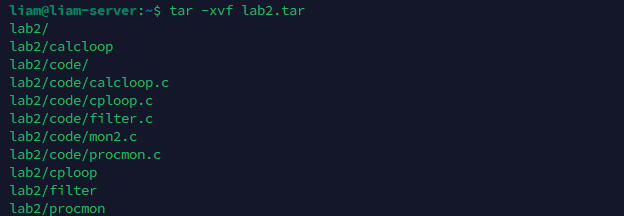
\includegraphics[width=0.8\textwidth]{./lab2_extraction.png}
    \caption{Extraction of \texttt{lab2.tar}.}
\end{figure}

\begin{figure}[h]
    \centering
    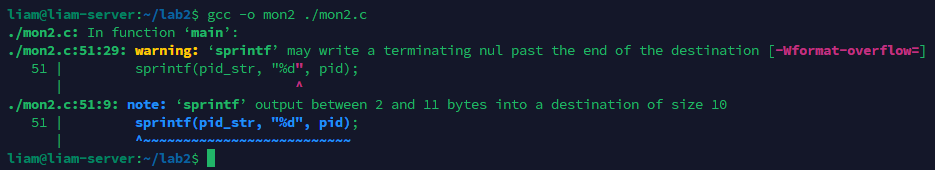
\includegraphics[width=0.8\textwidth]{./mon2_compilation.png}
    \caption{Compilation of \texttt{mon2.c}.}
\end{figure}

\begin{figure}[h]
    \centering
    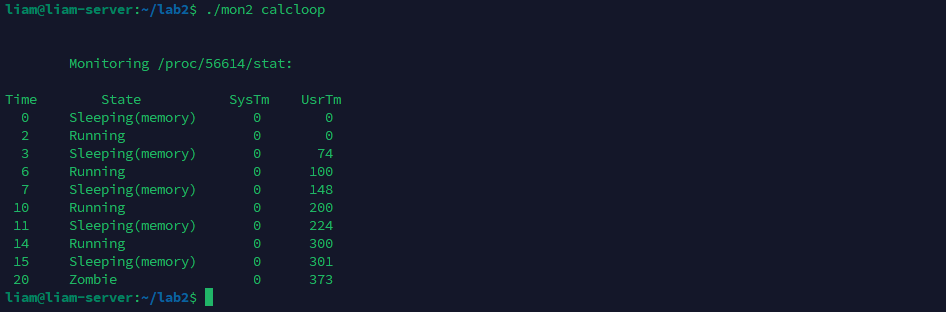
\includegraphics[width=0.8\textwidth]{./mon2_output.png}
    \caption{Execution of \texttt{mon2}.}
\end{figure}

\begin{figure}[h]
    \centering
    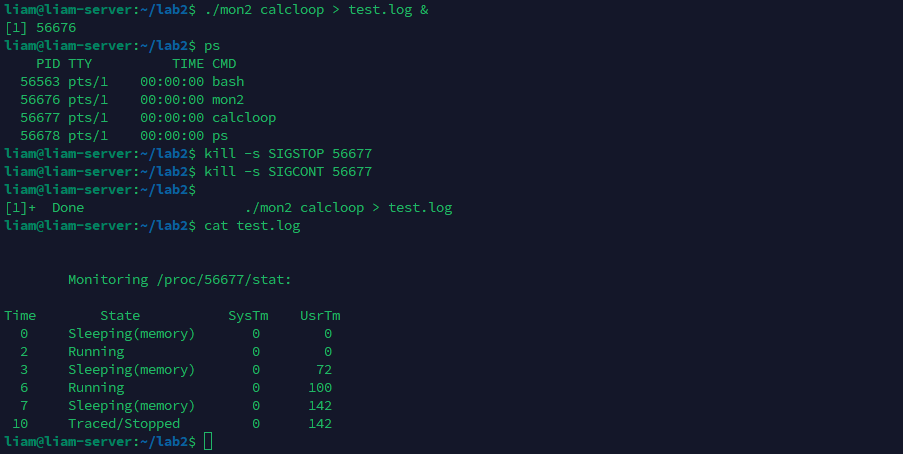
\includegraphics[width=0.8\textwidth]{./mon2_signals.png}
    \caption{Sending signals to \texttt{calcloop}.}
\end{figure}

\begin{figure}[h]
    \centering
    % \includegraphics[width=0.8\textwidth]{path/to/screenshot6.png}
    \caption{Compilation of Java files for Mandelbrot.}
\end{figure}

\begin{figure}[h]
    \centering
    % \includegraphics[width=0.8\textwidth]{path/to/screenshot7.png}
    \caption{Execution of \texttt{MandelBrot} with parameters.}
\end{figure}

\end{document}